% Don't number the intro chapter, but add it to the table of contents
% \addcontentsline{toc}{chapter}{Introduction}
% Doesn't seem like not numbering the intro chapter is a requirement, whereas it makes the subsection numbering weird
\chapter{Introduction}
\label{ch:intro}

\section{Cosmological big questions}

The glimpses of the Universe's most global behavior continue to surprise and fascinate us.
Early examples of such realizations include the expansion \citep{Slipher-extragalactic-radial-velocities,Hubbles-law} and vastness \citep{Hubble-extragalactic-distances}\footnote{Thanks to Leavitt's law \citep{Leavitt-law} for Cepheid variable stars enabling extragalactic distance measurements.} of the Universe.
Then, the discovery of accelerated expansion \citep{accelerated-expansion-perlmutter-et-al,accelerated-expansion-riess-et-al} was groundbreaking as well.
Now there are indications that the accelerating force may be weakening \citep{PantheonPlus-cosmo,Union3,DES-Y5-SN-cosmo,DESI2024.VI.KP7A,DESI.DR2.BAO.cosmo}.

The standard model of cosmology, $\Lambda$CDM, emerged soon after the discovery of the accelerated expansion of the Universe.
It had been remarkably successful in accommodating the different observations, but eventually some problems started to emerge.
One of the most famous is the Hubble ($H_0$) tension --- the more direct, local measurements of the current rate of expansion (most remarkably, from SH0ES collaboration, e.g. \cite{SH0ES}) give a value significantly larger than inferred from the cosmic microwave background (CMB, \cite{Planck2018-cosmo}).
% Another notable tension ($\sigma_8$ or $S_8$) relates to the slower growth of structure from galaxy lensing analyses as compared to CMB inference again.

Furthermore, $\Lambda$CDM bears two phenomenological ingredients in its name.
Constant dark energy ($\Lambda$) and cold dark matter (CDM) are the simplest possibilities for some fundamentally unknown substances thought to comprise $\approx 95\%$ of total density.
Cutting-edge measurements testing their properties can revolutionize our understanding of the Universe.

In this thesis, our major focus is on the expansion of the Universe: nature of its acceleration (mysterious dark energy) in \cref{ch:RascalC,ch:DESI-key} and discrepancy in the current speed inferred from different methods (Hubble tension) in \cref{ch:H0-clumping}.
Further, in \cref{ch:tSZ-selection-LRG} we explore how to extract even more information from our data, which should help to enlighten dark matter as well.

\section{Selected cosmological probes}

\subsection{Large-scale structure of the Universe: overview}

Galaxies (and matter) in the Universe are not distributed randomly \citep[e.g.,][]{distribution-of-galaxies-Shapley1933}.
On a relatively smaller scale, galaxies clump together in clusters and superclusters.
If we zoom out further, we can see that these groups follow a more global structure with filaments and walls -- the cosmic web.
This is the large-scale structure of the Universe.

In the $\Lambda$CDM model, the cosmic web is thought to form from tiny quantum fluctuations stretched by cosmic inflation, enhanced by gravitational collapse.
On the very largest scales (starting from hundreds of megaparsecs), the structure is assumed to be homogeneous (largely the same from any position) and isotropic (largely the same in any directions)\footnote{There are claims of observations indicating inhomogeneity or anistropy, although they have not been widely accepted.}.

\subsection{Galaxy surveys}

Measurements of the large-scale structure of the Universe through galaxies are one of the pillars of modern cosmology.
It provides access to the mass distribution\footnote{Not directly, because galaxies do not trace matter ideally.} of the Universe at different cosmic times.

The surveys systematically mapping galaxies on the sky come in two major varieties: photometric and spectroscopic.
Photometric observations (photometry) record the flux (luminous energy per area) in several filters (wavelength or frequency bands), which can be wider or narrower.
Spectroscopy provides finer details about the distribution of flux over wavelength (or frequency) of light; it can be loosely imagined as having a very high number of narrow, non-overlapping bands.

It generally takes more time or effort to obtain high-quality (high signal-to-noise ratio) spectroscopy than photometry of the same object, because the faint light is subdivided further.
Accordingly, spectroscopic observations often use more easily obtainable photometry to select targets for the optimal use of precious telescope and instrument time.

Spectra are particularly valuable in cosmology because they allow to obtain reliable redshifts.
Light propagating through the empty space is stretched (redshifted) together with the Universe.
In a good spectrum, one can identify a group of spectral emission or absorption lines with known atomic lines.
At least two lines are needed, because a single line can be almost anything with an unknown amount of stretching, whereas ratios of wavelengths (or frequencies) in pairs of lines are distinctive (if measured precisely enough) and do not change with an overall redshift.
The redshift is then the relative difference between the emitted and the observed wavelength (known based on laboratory measurements).
Redshifts add the third dimension to the more readily obtainable position on the sky (the 2-dimensional celestial sphere) and thus provide much more structural information.

There are methods of obtaining redshifts from photometry as well, but they are generally less reliable.
Improving these methods is an active area of research \citep[see e.g.][]{DES-Y3-redshift-calibration,photo-z-Dey2021,photo-z-Dey2022}.
For this reason, we do not explicitly use photometry in this thesis.

\subsection{Baryon acoustic oscillations (BAO)}

The early Universe was very hot and dense.
High abundance of energetic photons and frequent collisions kept the ordinary matter (colloquially called ``{\bf baryons}'' in cosmology\footnote{Which is loose by particle physics standards, because electrons are strictly not baryons but leptons. However, most of the mass of the ordinary matter is from baryonic particles --- protons and neutrons.}; mostly hydrogen) ionized.
Photons continually interacted with the ordinary matter (mainly through the free electrons), so that they all were in common equilibrium, comprising so-called photon-baryon plasma.
Photons provided relativistically high pressure in this mixture, preventing the gravitational collapse of baryons and instead enabling sound waves ({\bf acoustic oscillations}) propagating at roughly $1/\sqrt{3} \approx 0.58$ speed of light.

As the Universe expanded, it was diluting and becoming colder.
Gradually, the photon-baryon interactions became much rarer and weaker, allowing neutral (hydrogen) atoms to form from ions and free electrons in a process called cosmic {\bf recombination}\footnote{``Combination'' might be a better name because the ions and electrons had never combined at an earlier point in cosmic history, to the best of our current knowledge. But the term was formed in other circumstances, in which ``re-'' was appropriate, and borrowed to cosmology.}, which further decreased the collision frequency in a feedback loop.
As a result, eventually the photons and baryons went their separate ways: photons propagated (almost) freely, and baryons collapsed to form galaxies in the cosmic web (not just by themselves but also into the potential wells already formed by dark matter, which was not deterred by photon pressure).
Still, the acoustic oscillations are imprinted in both --- mostly as it is more likely to find two higher (or two lower) densities at a distance that the sound waves traveled between the Big Bang and the recombination (the {\bf sound horizon}, which can be computed theoretically, including numerical models).
\citep[This description largely follows][.]{Sunyaev-Zeldovich-1970,Peebles-Yu-1970}

The acoustic oscillation feature is weaker in baryons than in primordial photons.
This is because the subsequent evolution of ordinary matter was more influenced by the gravitational interaction with the dark matter, which was largely unaffected by the photon pressure.
But despite this and other complicating effects, it remains slightly more likely to find galaxies at the sound horizon distance from each other than at other similar distances, and this picture stretches with the expanding Universe (is largely preserved in cosmological comoving coordinates).

Thus, baryon acoustic oscillations provide a (comoving) standard ruler.
Dividing the real size (sound horizon) by the angular size of the feature as observed on the sky gives the (comoving) angular diameter distance\footnote{Comoving angular diameter distance is also called the transverse comoving distance.} by definition.
This distance is then related to the integrated rate of the expansion of the Universe between now and then\footnote{And the spatial curvature of the Universe if we do not assume its absence on the largest scales.}.
This measurement is called transverse BAO.

Redshift measurements also provide an additional measurement in the third dimension (line-of-sight BAO).
The change in cosmological redshift is connected to the line-of-sight distance interval via the momentary rate of the expansion of the Universe.
This way, measurement of the size of the BAO feature in redshift space and knowledge of the real size (sound horizon) gives the expansion rate at the representative time for the observed galaxy sample.

Without the absolute size of the sound horizon, BAO measurements with different galaxy samples can provide relative distance measurements to different redshift times and thus constrain the relative dynamics of the expansion of the Universe, but not its absolute rate.

\subsection{Cosmic microwave background (CMB)}

The cosmic microwave background is the oldest light that can be observed, often called an afterglow of the Big Bang.
It is formed of photons propagating freely after last interacting with (scattering on) matter during cosmic recombination.
They cooled down due to stretching with the expanding Universe to the typical millimeter (roughly microwave) wavelength.
It is an on-sky image of predominantly a thin spherical shell of the Universe (surface of last scattering), from which photons originating at the times of recombination could reach us now by going straight all the time in between.

The CMB is famously an almost ideal example of blackbody (thermal) radiation with very nearly identical temperature ($T\approx 2.725$~K) in all directions.
After the subtraction of the dipole, which can not be disentangled from the motions of the Earth and its surroundings, the differences are tiny at $\lesssim 100~{\rm \mu K}=10^{-4}~$K.
We show the map of these fluctuations in \cref{fig:cmb-map}.
CMB also has similarly small polarization variations across the sky.
Such small perturbations can be modeled and interpreted very precisely and robustly, and they provide a great view of the early Universe.

\begin{figure}[htb]
    \centering
    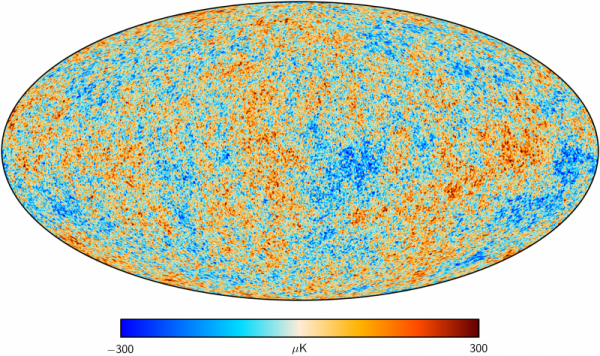
\includegraphics[width=\textwidth]{img/planck_int_cmb_0.png}
    \caption{Map of the cosmic microwave background (CMB) temperature fluctuations measured by the {\it Planck} satellite. (Image credit: ESA and the Planck Collaboration.)}
    \label{fig:cmb-map}
\end{figure}

\begin{figure}[hbt]
    \centering
    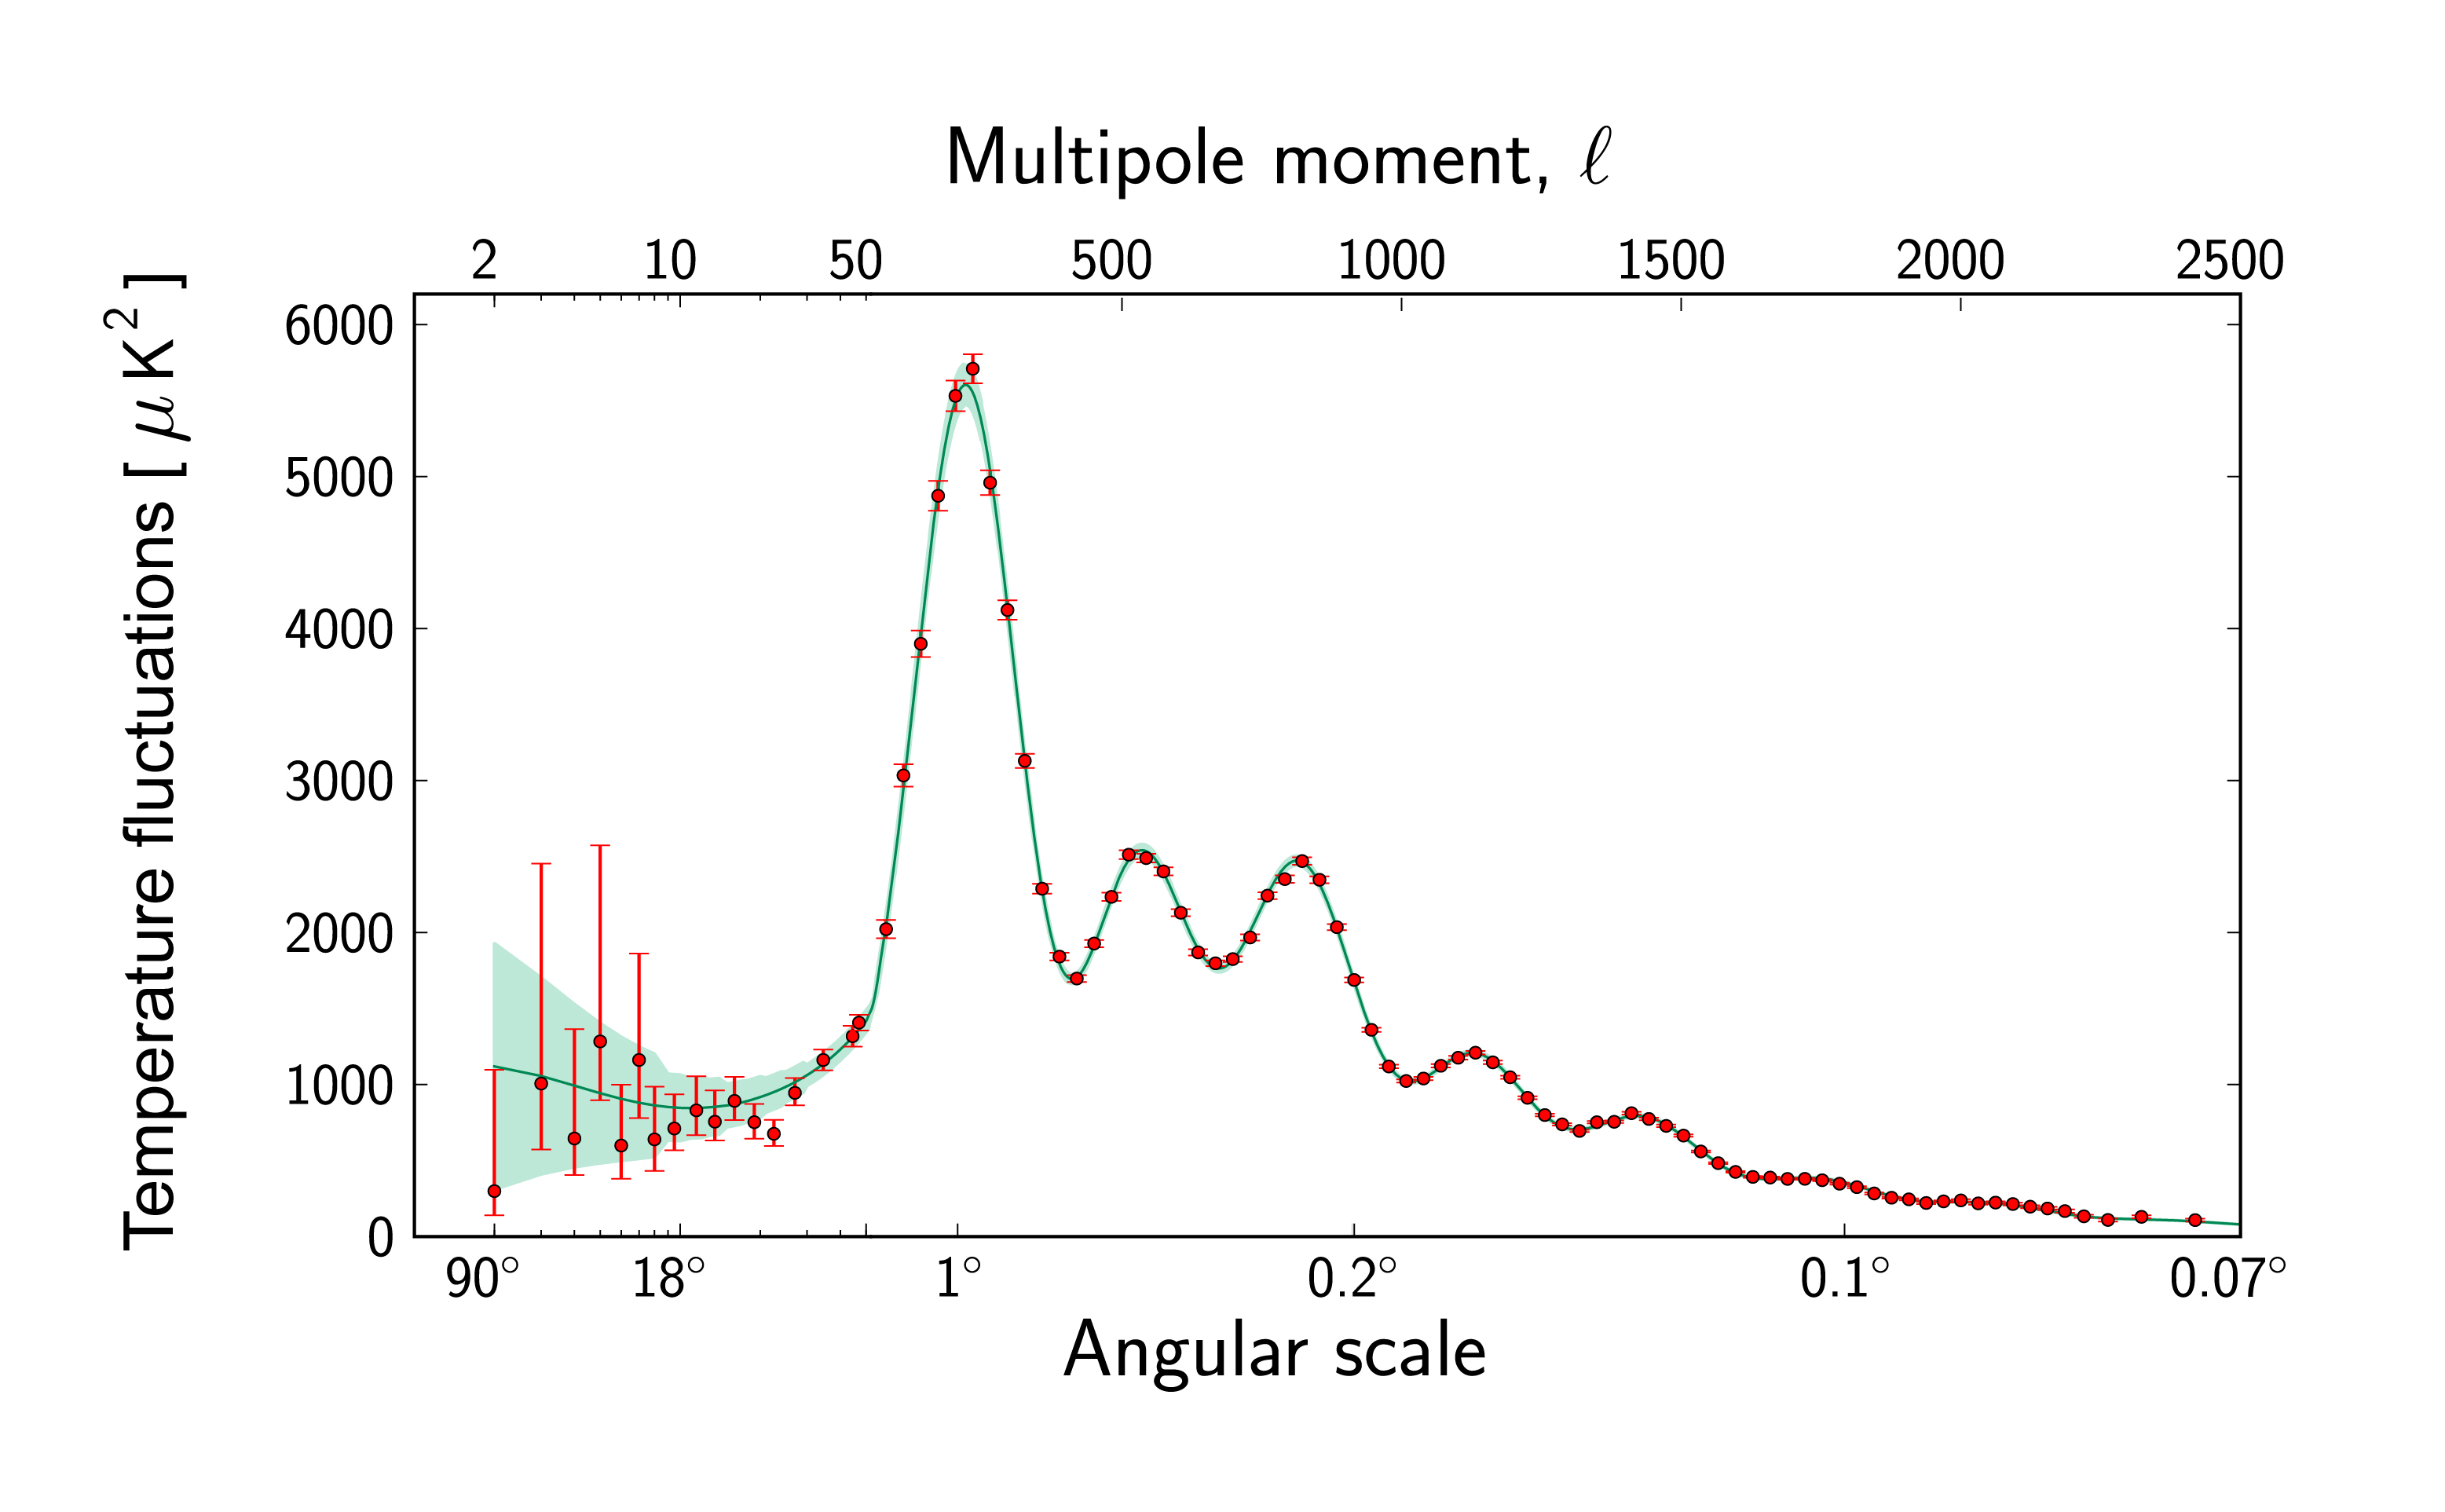
\includegraphics[width=\textwidth]{img/Planck_Power_Spectrum.jpg}
    \caption{Cosmic microwave background (CMB) temperature power spectrum measured by the {\it Planck} satellite (red dots with errorbars) and predicted by the $\Lambda$CDM model (green). (Image credit: ESA and the Planck Collaboration.)}
    \label{fig:cmb-power-spectrum}
\end{figure}

The maps of CMB fluctuations are summarized by angular power spectra.
The angular power spectrum is a statistical tool describing the amount of variations on different angular scales.
We show the CMB temperature power spectrum in \cref{fig:cmb-power-spectrum}.

Several features are apparent in \cref{fig:cmb-power-spectrum}.
One can see the damped oscillations with the first peak at an angular scale $\sim 1^\circ$.
The period of these oscillations, measured very precisely, is set by the acoustic feature we described in the previous section, analogous to the transverse BAO in galaxies.
The damping is due to photon diffusion before and during the cosmic recombination \citep[the process known as Silk damping,][]{silk-damping}.
The additional height variations in the oscillatory peaks are regulated by the amount of ordinary matter (baryons).

The formation of the CMB was intertwined with the evolution of the large-scale structure.
E.g., through gravitational interaction with dark matter, including gravitational redshift from maxima and minima of the gravitational potential.
CMB also has secondary anisotropies, formed by photons' interaction with matter after recombination, on their way towards us.
These include gravitational lensing (deflection by masses of dark matter and baryons) and scattering on re-ionized baryon gas (Sunyaev-Zeldovich effect, which we will use in \cref{ch:tSZ-selection-LRG}).

\subsection{Standard candles: Type Ia supernovae}

The standard candle is an object with a fixed luminous power (total or in a certain wavelength range).
By knowing this power and measuring the power per area we receive from the object, we can compute the distance using the inverse-square law.
More precisely, in cosmology, this gives a luminosity distance, which is related to the integrated rate of the expansion of the Universe between now and the emission of the light, like the other distances.

Supernovae of a distinct type (Ia) are nearly standard candles.
They have been identified with a certain subclass of explosions of white dwarfs exceeding the Chandrasekhar limit by accretion.
Type Ia supernovae provided one of the first definite pieces of evidence in favor of accelerated expansion of the Universe \citep{accelerated-expansion-perlmutter-et-al,accelerated-expansion-riess-et-al}.

For precision cosmology with Type Ia supernovae, it is necessary to go beyond the assumption of constant intrinsic power by establishing connections with other observable quantities starting from the rate of luminosity decrease (Phillips relation).
Technically, this makes them standardizable candles.
The light can also be partially obscured, e.g. by cosmic dust.
Many of the necessary corrective relations are not understood from first principles and need to be calibrated using other distance measurements.
An additional complication is that Type Ia supernovae are relatively rare and have hardly been observed within the reach of more direct distance measurements (parallax), thus, the calibration has to rely on a different type of standardizable candles, e.g., Cepheid variable stars.
This thesis does not include original work on details of these measurements in particular, so we refer a curious reader to \cite{SH0ES-2022,CCHP-status-report-Freedman,PantheonPlus-cosmo,Union3,DES-Y5-SN-cosmo}.

\section{Dark Energy Spectroscopic Instrument (DESI)}

The Dark Energy Spectroscopic Instrument \citep[DESI,][]{DESI2016a.Science} is conducting a major spectroscopic galaxy survey since 2021.
The instrument \citep{DESI2016b.Instr,DESI2022.KP1.Instr} takes approximately 5000 spectra simultaneously.
To deliver light to the spectrographs, it uses optical fibers individually positioned by miniature robots in the focal plane of the 4-meter Mayall telescope at Kitt Peak, Arizona.
This allows to change the configuration quickly and automatically to targets selected in advance.
The target selection relies on photometric Legacy Imaging Surveys \citep{LS.Overview.Dey.2019}.

During the main 5-year program, DESI is scheduled to cover 14,000 square degrees on sky and the redshift range $0<z<3.5$.
As a result, the DESI survey will surpass the previous leading surveys (mainly SDSS/BOSS/eBOSS) by an order of magnitude in both volume and number of extragalactic objects, collecting more than 30 million galaxy and quasar spectra.
One of the main scientific drivers for its design was the precision of the BAO measurements.

\section{Statistics of the Universe on large scales}

In this chapter, we provide a slightly deeper review of the statistical methodology used to describe the large-scale structure.

\subsection{Overdensity field}

By field, we mean assignment of a value (e.g., a number or a vector) to each point in space (and time).
In the standard cosmological paradigm, we assume that the initial conditions are set randomly (stochastically) by the quantum fluctuations during cosmic inflation.
Accordingly, we treat our observables as random fields.

Having a mass density field, we define a mass overdensity at any point:
\begin{equation}
    \delta \qty(\vec x) \equiv \frac{\rho \qty(\vec x)}{\bar \rho} - 1 \label{eq:mass-overdensity}
\end{equation}
The average density depends on cosmic time.
However, measuring the mass density in 3 dimensions can be incredibly hard.

In galaxy surveys, we instead observe galaxies mainly as points with a certain position.
We can talk about their number density --- number per volume.
Ideal points can be represented with Dirac delta functions $\delta^D \qty(\vec x - \vec x_p)$, which, integrated over a volume, indicate 0/1 whether a point is inside or not.
Alternatively, one might imagine a fine grid of cells, each of which has a volume and a number of galaxies (possibly 0) and thus an average density.

From the number density, we define the number overdensity
\begin{equation}
    \delta \qty(\vec x) \equiv \frac{n \qty(\vec x)}{\bar n} - 1 \label{eq:number-overdensity}
\end{equation}
Points can be weighted; that should be taken into account in the average density.
Also, the average density for a real galaxy survey should reflect the selection effects.

Because either density is non-negative, for either overdensity $\delta \qty(\vec x) \ge -1$.
By design, $\ev{\delta \qty(\vec x)} = 0$, averaging over the possible realizations of the Universe from the random quantum fluctuations.

We can also describe the overdensity field as a sum of plane waves (Fourier modes) $\delta \qty(\vec k)$ with wavevector $\vec k$ using a Fourier transform:
\begin{align}
    \tilde \delta \qty(\vec k) &\equiv \int d^3 \vec x\, \delta \qty(\vec x) e^{-i \vec k \cdot \vec x} \label{eq:overdensity-fourier} \\
    \delta \qty(\vec x) &= \int \frac{d^3 \vec k}{\qty(2\pi)^3} \tilde \delta \qty(\vec k) e^{i \vec k \cdot \vec x}.
\end{align}
Space of wavectors $\vec k$ is commonly referred to as Fourier space, and the space of coordinates $\vec x$ --- as configuration space; the two descriptions are equivalent.

The Fourier image is convenient because linear equations give an independent time evolution of different Fourier modes (plane waves).
And linear equations are a great approximation for small perturbations.

\subsection{Gaussian random field}

A Gaussian random field is a random field in which the joint distribution of values at any number of points is a multivariate normal (Gaussian) distribution.
It is a convenient and common abstraction or approximation in cosmology.

First and foremost, we mean the distribution of possible realizations of the Universe from primordial quantum fluctuations.
But with homogeneity and isotropy, the spatial distribution on large scales should approach it (akin to the ergodic hypothesis).

Assuming translation invariance (homogeneity), a Gaussian random field can be obtained as a sum of independent Fourier modes.
% Inverse should be true as well.
Fourier modes of a Gaussian random field also represent a Gaussian random field in Fourier space.

The early Universe is very close to Gaussian, as predicted from the inflationary foundation of $\Lambda$CDM and seen in the CMB maps \citep[e.g.,][]{planck_overview}.
As we remarked before, linear evolution preserves the mode independence and thus Gaussianity.
Later evolution by gravity and other interactions on small scales causes deviations (non-Gaussianity).
Because different modes start to affect each other's evolution when perturbations grow beyond linear.
Another, simpler reason is that a normal distribution with zero mean and large deviations (dispersion, variance) strongly violates $\delta \qty(\vec x) \ge -1$.
Primordial non-Gaussianity is also possible (e.g., predicted by some inflation models), and active search is ongoing using CMB \citep[e.g.,][]{Planck18-PNG} and LSS data \citep[e.g.,][]{local-PNG-DESI-LRG-photometric,ChaussidonY1fnl}.

A normal (Gaussian) distribution is completely determined by its mean and covariance.
As we remarked in the previous section, cosmic overdensity fields have zero mean by construction.
This leaves the covariance, the pairwise correlations.
With (large-scale) homogeneity, they can depend only on the vector between the points.
With isotropy, only distance matters.
But the line-of-sight direction is different from the others (e.g., in redshift-based distance determination), so the angle with it matters too.

A Gaussian random field shares a convenient property with the normal distribution.
Isserlis' theorem\footnote{Isserlis' theorem is also known in particle physics and cosmology as Wick's (probability) theorem after \cite{Wicks-theorem}.} \citep{isserlis} states that with zero mean, all higher moments (correlations of higher-point) are determined by the covariance (2-point correlations).
In particular, the odd-order (odd-point) quantities are zero.

\subsection{The 2-point correlation function (2PCF)}

The 2-point correlation function (2PCF) of discrete particles (e.g., galaxies or dark matter halos) describes the excess probability of finding two such particles separated by a certain distance, compared to the random scatter case.
\begin{equation}
    \xi \qty(\vec r) = \frac{dP_g(\vec x_g + \vec r | \vec x_g)}{\bar n \cdot d^3 \vec r} - 1. \label{eq:2PCF-discrete-probability}
\end{equation}
$dP_g(\vec x_g + \vec r | \vec x_g)$ is the conditional probability of finding a (different) galaxy in an infinitesimal volume $d^3 \vec r$ around $\vec x_g + \vec r$ given a galaxy at $\vec x_g$.
$\bar n$ is again the expected number density if the Universe were unclustered; it should reflect the survey selection effects, weighting scheme, etc.

Perhaps a more intuitive statement is that the probability of finding two particles (e.g., galaxies or halos) in infinitesimal volumes $d^3\vec x_{1,2}$ near $\vec x_{1,2}$ respectively is
\begin{equation}
    dP_{12} = \bar n d^3\vec x_1 \cdot \bar n d^3\vec x_2 \cdot \qty[1+\xi\qty(\vec x_2 - \vec x_1)],
\end{equation}
where we can set $\vec r \equiv \vec x_2 - \vec x_1$.

A more general definition of the 2PCF is through the spatial correlations of overdensities (\cref{eq:mass-overdensity} or \cref{eq:number-overdensity}):
\begin{equation}
    \xi \qty(\vec r) = \ev{\delta \qty(\vec x) \delta \qty(\vec x + \vec r)} = \frac1V \int d^3 \vec x \delta \qty(\vec x) \delta \qty(\vec x + \vec r). \label{eq:2PCF-overdensity}
\end{equation}
For the number overdensity of discrete particles (\cref{eq:number-overdensity}) this definition is theoretically equivalent to the probabilistic one (\cref{eq:2PCF-discrete-probability}).

BAO feature manifests as a peak of the correlation function (scaled by $r^2$) at $r\approx 150$~Mpc. %$\approx 100\ihMpc$.
This feature is relatively subtle and requires large galaxy samples to detect.
The first discovery this way was in \cite{BAO-discovery-Eisenstein-et-al}.

2PCF can be estimated by counting pairs between observed galaxies (data) $D$ and random points $R$  distributed according to the background density $\bar n$.
Therefore, randoms reflect the survey boundaries, subtler selection effects and weighting.
It is often more efficient to generate random points than to write some functional form of $\bar n(\vec x)$.

The probabilistic definition (\cref{eq:2PCF-discrete-probability}) motivates the Davis-Peebles estimator \citep{Davis-Peebles}:
\begin{equation}
    \hat \xi_{\rm DP} \qty(\vec r_{\rm bin}) = \frac{DD\qty(\vec r_{\rm bin})}{DR\qty(\vec r_{\rm bin})} - 1,
\end{equation}
where $DD\qty(\vec r_{\rm bin})$ is the (weighted) count of pairs of data points with separation $\vec r$ between them belonging in a certain region (bin) around $\vec r_{\rm bin}$, and $DR\qty(\vec r_{\rm bin})$ is the same but for data-random pairs.

Expansion of the correlation function through overdensities (\cref{eq:2PCF-overdensity,eq:number-overdensity}) motivates the Landy-Szalay estimator \citep{Landy-Szalay}:
\begin{equation}
    \hat \xi_{\rm LS} \qty(\vec r_{\rm bin}) = \frac{DD\qty(\vec r_{\rm bin}) - 2 DR\qty(\vec r_{\rm bin}) + RR\qty(\vec r_{\rm bin})}{RR\qty(\vec r_{\rm bin})},
\end{equation}
where $RR\qty(\vec r_{\rm bin})$ is the same as $DD$ and $DR\qty(\vec r_{\rm bin})$ but counting pairs of random points.
The Landy-Szalay estimator has minimal variance and is more stable to small fluctuations in the random points \citep{2PCF-estimator-comparison-Kerscher}, so we rely on it exclusively in \cref{ch:RascalC,ch:DESI-key}.
At the same time, the Davis-Peebles estimator is less demanding in multiple ways, one of which is important in \cref{sec:DESI-tSZ:measurements:methodology}.

\subsection{The power spectrum}

The power spectrum is defined through the correlation of the Fourier modes (\eqref{eq:overdensity-fourier}):
\begin{equation}
    \ev{\tilde \delta \qty(\vec k) \tilde \delta^* \qty(\vec k')} = \qty(2\pi) P(\vec k) \delta^D \qty(\vec k - \vec k'), \label{eq:Pk-definition}
\end{equation}
where $\delta^D$ is the Dirac delta function, theoretically infinite at zero argument and zero elsewhere.
In practice, power spectrum estimation uses a finite volume with a discrete Fourier transform, which transforms the Dirac delta function (infinite at zero) with a volume multiplier if and only if $\vec k = \vec k'$ (technically, Kronecker delta).

The BAO feature manifests as a series of peaks in the power spectrum.
This was first measured in data by \cite{BAO-discovery-Cole-et-al}.

The 2-point correlation function and the power spectrum are connected via the Fourier transform:
\begin{align}
    P \qty(\vec k) &= \int d^3 \vec r \, \xi \qty(\vec r) e^{-i \vec k \cdot \vec r} \\
    \xi \qty(\vec r) &= \int \frac{d^3 \vec k}{\qty(2\pi)^3} P \qty(\vec k) e^{i \vec k \cdot \vec r}
\end{align}
Thus, 2PCF and power spectrum contain identical information if measured over infinite ranges.
However, a cut in Fourier space does not correspond to a cut in configuration space and vice versa.
Additionally, survey geometry and selection effects are more complicated for the power spectrum \citep{pypower-methodology}.

\subsection{Higher-point statistics}

Higher-point statistics can be obtained by generalizing \cref{eq:2PCF-overdensity,eq:Pk-definition}.
E.g., the 3-point correlation function:
\begin{equation}
    \zeta \qty(\vec r_1, \vec r_2) = \ev{\delta \qty(\vec x) \delta \qty(\vec x + \vec r_1) \delta \qty(\vec x + \vec r_2)}
\end{equation}
and the bispectrum (the Fourier-space 3-point function):
\begin{equation}
    \ev{\tilde \delta \qty(\vec k_1) \tilde \delta \qty(\vec k_2) \tilde \delta^* \qty(\vec k_3)} = \qty(2\pi) B(\vec k_1, \vec k_1) \delta^D \qty(\vec k_1 + \vec k_2 - \vec k_3)
\end{equation}

As we mentioned before, for a Gaussian random field, higher-point statistics are set by the 2-point statistics \citep{isserlis}.
For a non-Gaussian field, they contain additional information, approaching completeness as order increases to infinity.
However, the information content does not increase very fast, whereas the number of dimensions grows quickly (even after one uses additional symmetries to reduce dimensionality).
This motivates the search for alternatives.

\section{Large-scale structure data analysis and covariance matrices}

For meaningful (statistical) interpretation of data (Bayesian or frequentist), it is crucial to compute the likelihood --- describing the probability of obtaining the data given a model.
Fortunately, the distribution of measured clustering statistics is well described by a multivariate Gaussian (thanks to the central limit theorem and typically averaging a large number of modes), which is fully described by the mean and the covariance matrix.
The mean can be set to the theoretical prediction, which leaves the covariance.

Perhaps the most intuitive approach to the covariance is scatter in repeated independent measurements.
However, repeating a cutting-edge survey even once more is hardly practical.
Moreover, the fact that we have only one Universe sets a limit to how many big surveys (covering the same redshifts) can be done before they have to overlap.

The next option is simulating the Universe in computer models (ultimately, making mock galaxy catalogs).
This solution is far from ideal.
Detailed simulations are computationally expensive, more so as they need to cover larger volumes for bigger surveys.
A precise covariance estimate requires a large number of samples, increasingly higher as more quantities are measured.
This forces a hard compromise between quality and quantity, keeping the total computation time very long.
Such catalogs need to capture key aspects of clustering and be representative of the data or the assumed theoretical model.
The mock-based covariance production is therefore not characterized by flexibility, as the generation and processing of numerous simulations for an updated dataset or alternative model requires a huge effort.

Another method involves making multiple samples by selecting different subsets of the data.
The lack of dependence on mocks and model assumptions makes them attractive.
These are represented by resampling techniques like jackknife and bootstrap, which involve splitting the data into parts.
However, it is often hard to divide an intricately shaped survey volume into equivalent regions.
These regions would not be independent of each other because large-scale correlations exist.
Subsets of the survey may have more complicated boundaries, affecting the covariances in ways not described by simple scalings.

From a theoretical point of view, covariance of 2-point functions (\eqref{eq:2PCF-overdensity}) involves expectation values at 4 points.
In a Gaussian random field, by Isserlis' theorem \citep{isserlis}, they can be reduced to 2-point functions between different pairs of points.
The 2-point function could be measured from the data or modeled theoretically and substituted into its covariance computation.
However, non-Gaussianities develop over cosmic time.
Galaxies correspond to high matter overdensities, evolving in a crucially nonlinear regime.
This makes the derivation of important higher-point corrections to the ideal Gaussian picture also very challenging.
Measuring the necessary 3- and 4-point functions from the data reliably is hard as well because of the large number of bins needed.

Each of these approaches has its advantages and disadvantages.
It would be nice to develop an optimal combination.
This is what we approach in a major part of this thesis, \cref{ch:RascalC}, by combining theory with data resampling (or simulated Universes).

\section{Outline of the thesis}

\cref{ch:RascalC} is dedicated to the important technical work on the fast semi-theoretical, semi-empirical covariance matrices for 2-point correlation functions.
\cref{ch:DESI-key} then shows a selection of global DESI BAO results, which relied on these covariance matrices (along with multiple other supporting studies).
We focus on the nature of dark energy and the Hubble tension.
\cref{ch:H0-clumping} follows with our earlier work on a potential relief of the Hubble tension through inhomogeneous recombination, which does not require fundamentally new physics.
\cref{ch:tSZ-selection-LRG} presents our work in progress on extracting more information than standard 2-point functions allow without higher-point functions, by using the DESI spectroscopic galaxies together with secondary CMB anisotropies maps.
In \cref{ch:conclusion} we reflect on the achieved results and discuss future directions.